\header{
    \headtitle{L'hymne Juriste Grenoble} \label{l-hymne-juriste-grenoble}
    %%
    
    \insertComment{Sur l'air de "L'artilleur de Metz".}{}
}

\enluminure{4}{\href{https://www.youtube.com/watch?v=vPyXuK2r91E}{Q}}{uand} les juristes soiffards
\\Arrivent dans un bistrot,
\\Les barmans pères peinards
\\Les traitent d'alcoolos.
\\Pour ne pas contrarier
\\Ces pauvres cafetiers,
\\Les juristes vont se murger
\\Et sans dégobiller.
\begin{tikzpicture}[remember picture,overlay]
    \node[xshift=-4cm,yshift=-7.5cm] at (current page.north east){%
    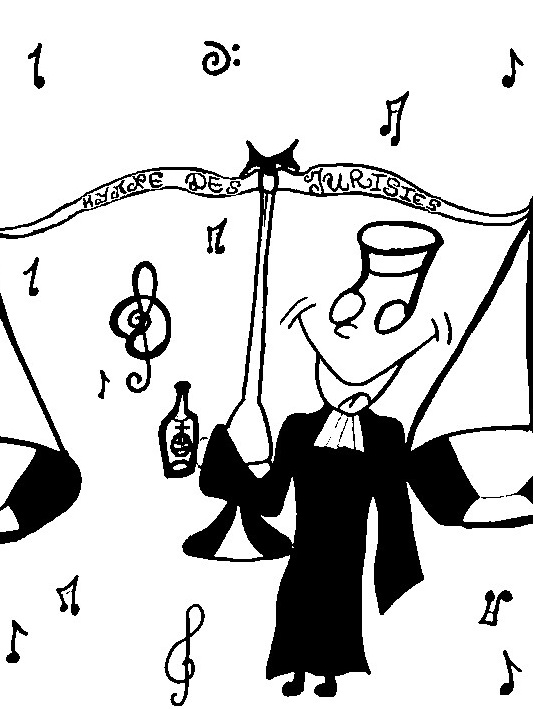
\includegraphics[width=0.3\textwidth]{images/hymne_juriste.jpg}};
\end{tikzpicture}
\\\\\textbf{Refrain : }
\\Aux juristes chers frères,
\\A la justice levons un verre,
\\Et répétons ce beau refrain,
\\Viv' les procès, le sexe et les pots de vin.
\\\textit{(seul)} Et répétons ! \textit{(tous)} Et répétons !
\\\textit{(seul)} Ce beau refrain ! \textit{(tous)} Ce beau refrain !
\\\textit{(ensemble)} Viv' les procès, le sexe et les pots de vin
\dualcol{
    Tous les juristes sont beaux
    \\Avec leurs corps d'athlètes,
    \\Leurs muscles, leurs pectoraux
    \\Et puis leurs goûts d'esthètes.
    \\En plus intelligent,
    \\Mais aussi amusant,
    \\Les femmes se disent à quand
    \\Un juriste pour amant
    \\\\A l'appel des donzelles,
    \\Le satin rouge s'immisce
    \\Et toutes les jeunes pucelles
    \\Se ruent vers les juristes.
    \\Une fois qu'elles en tiennent un,
    \\C'est pour leur faire du bien
    \\Qu'il glisse entre leurs reins
    \\La pine dans leur vagin.
    \\\\Un juriste ça vaut bien
    \\Plus de dix carabins
    \\Qui sont des bons à rien
    \\Tout comme les pharmaciens.
    \\Ils nous font rigoler,
    \\Ces pauvres épiciers, adieu-fais-toi-putain
}

\breakpage